\section{Problem statement}
\label{problem_statement}

In this section, the problem is formally defined after a few fundamental concepts are formally defined.

%% Formal definition of relational table
\begin{definition}[Relational table]
    Given a set of $n$ domains $D = \{D_1, D_2, ..., D_n\}$, a \emph{relational table} $R(A:d_1, B:d_2, ...)$ is defined on these $n$ domains as a subset of the Cartesian product of $D$, where a domain $d_i \in D$ is the set of possible values that a data element may contain \cite{codd_db}.

    \begin{equation}
    \begin{aligned}
    R(A:d_1, B:d_2, ...) \subseteq \times \{D_i : i=1, 2, ..., n \}
    \end{aligned}
    \end{equation}
    
    The notion $R(A:d_1, B:d_2)$ denotes a relational table made of two \emph{attributes} $A$ and $B$ taking values respectively from domain $d_1$ and $d_2$, i.e. $A \in d_1$ and $B \in d_2$. 

\end{definition}

%% Formal definition of query
\begin{definition}[Query]   \label{def:query}
    A user can retrieve information from a relational table by sending a \emph{query} which is nothing more than a set of conditions over the possible attributes. A query $q$ is formally defined as a function taking as input a set of conditions $C$ over the attributes of the relational table $R$, returning a subset of tuples of $R$ that satisfy the conditions in $C$; the queries are assumed to be defined as a set of conjunctions, i.e. 
    \begin{equation}
    \begin{aligned}
    q(C) \coloneqq \bigwedge_{c_i \in C} c_i
    \end{aligned}
    \end{equation}
        
    Throughout the entire paper, the set of all the queries will be referred to as $Q$. 
    
\end{definition}

%% Formal definition of rating function
\begin{definition}[Rating function]
    Before defining the problem it's important to define the concept of rating function. A \emph{rating function} $r$, which is a specialized version of the utility function described in the related work section, associates users taken from a set of users $S$ and queries taken from a set of queries $Q$ with ratings in the range $1-100$. A rating is the means by which a user expresses his opinion regarding the outcome of a query: a rating of $1$ denotes that the result of the query is unsatisfactory, whereas a rating of $100$ denotes that the result satisfies the user. 
    \begin{equation}
    \begin{aligned}
    r \colon S \times Q \to \mathbb{N} \in [1,100]
    \end{aligned}
    \end{equation}
    
    A rating function facilitates the definition of a \emph{utility matrix} $U$, which is a $|S| \times |Q|$ matrix containing for each cell $U_{ij}$ a rating in range $1-100$ if the user $i \in S$ has rated query $j \in Q$, otherwise $U_{ij}$ will be empty. 
\end{definition}


%% TODO: formalize the definition of recommendation system



%% Formal definition of the problem
\begin{definition}[Problem statement]
    Given the following inputs
    \begin{itemize}
        \item a relational table $R$ defined on a set of possible domains
        \item a set of users $S$
        \item a set of queries $Q$
        \item an utility matrix $M$, defined according to the aforementioned rating function $r$
    \end{itemize}
    fill in all the blanks in the utility matrix $M$ in such a way that if a user $i \in S$ would likely appreciate the result of query $j$, the corresponding rating $U_{ij}$ in the utility matrix should be filled with a positive rating. In the same way, the rating $U_{ij}$ associated with user $i$ should be negative if it is likely that the user will not appreciate the result of query $j$. 
    %Objective of the problem statement
    The objective is to use the utility matrix information to provide query recommendations to users based on their preferences. In fact this method can be used for finding the most promising queries that the user hasn't rated but that may be of interest to him. 

\end{definition}


\begin{definition}[Problem statement - Part B]
    Given as input
    \begin{itemize}
        \item the utility matrix $M$, filled with all the missing ratings
        \item a generic query $q$, defined as a conjunction of conditions as shown in Definition \ref{def:query} 
    \end{itemize}
    compute the importance of the query $q$ according to how important the query is to the individual users, by taking into account the ratings each user has already given to other queries, as specified by the utility matrix $M$.
\end{definition}


%% General idea
The general idea is to build a sophisticated query recommendation system to be integrated in a DBMS in order to take advantage of similarities in user ratings to recommend queries to other users based on the aforementioned inputs. Figure \ref{fig:workflow} accurately depicts the workflow of the recommendation system, which involves a user sending a query to a database through a DBMS, which then retrieves some data from it. Once the user receives the query result, he chooses to provide a rating. Based on those ratings, the recommendation system gives back to the user some recommendations.


\begin{figure}[h]
    \centering
    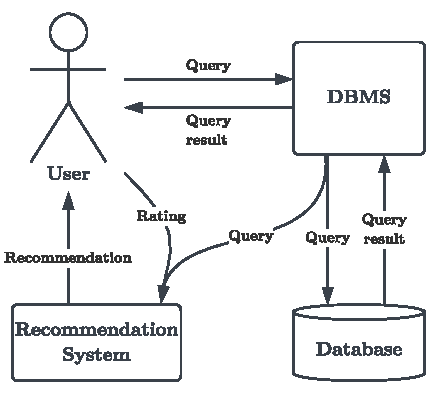
\includegraphics[width=0.30\textwidth]{imgs/architecture.pdf}
    \caption{\normalfont The workflow of the query recommendation system}
    \label{fig:workflow}
\end{figure}